\section{Method}
In the two sections below the methods adopted for respectively creating a residual map and for classification of NIR-dropouts are described.

\subsection{Producing a Residual Map with Profile-Fitting}
Since we are interested in objects that are visible in the IRAC bands and not visible in the NIR bands, we aim to produce a residual map of the IRAC $ch1$ image. However, due to limited computing power we refrain from attempting to create a residual map of the entire IRAC image, the full extent of which is $5.2$ arcmin$^2$. Instead we will work with tile 7-7, which is a smaller region in the image, spanning $\sim 8$ arcsecond$^2$. \\
In general a residual map is produced by creating a model of the image and subtracting it from the scientific image. To produce a model of the entire image one first needs to perform source detection, so it is known which objects that should be subtracted. Furthermore, one need to apply either aperture photometry or model-based photometry, which is in general terms a way of estimating the flux from a source, so we can subtract appropriate values from the scientific image. The details of the steps described here, are elaborated in the subsections below.

\subsubsection{Source Detection and Aperture Photometry}
In the COSMOS2020 Classic catalogue, the object photometry is carried out using SEP \cite{SEP_2018}, a Python wrapper for SExtractor \cite{SExtractor_1996}. To understand how the software works, we performed the source detection on the telescope images from three bands: two optical bands ($g$ and $i$) from the Hypersurprime Camera (HSC) mounted on \textit{Subaru} and the NIR band $Ks$ from VISTA. The code is available in this notebook \href{https://github.com/KimiKreil/Bachelor_Thesis_Code/blob/main/Code/Source_Detection.ipynb}{(link)}.
First, we need to produce background estimation, since each pixel in a telescope image is the sum of background noise and flux from the object that we are interested in. The background estimation is a way of mapping the background flux level in different areas of the image. Subtracting this background map, we can thus produce a "clean" image, where the background is $\sim 0$ so the pixel flux values within a source on average only includes the flux we are interested in. There will still be statistical fluctuations present. \\
\begin{wraptable}{r}{0.35\textwidth}
    \begin{tabular}{lc}
    \hline
    \textbf{Camera} & \textbf{Zero Point [mag]} \\ \hline
    HSC &  31.4 \\ 
    VISTA &  30 \\ 
    IRAC &  21.58 \\ \hline
    \end{tabular}
    \caption{Zero point magnitudes to convert flux  densities (in the image's native units) into magnitudes for the listed bands.}
    \label{zero_point}
\end{wraptable}
There are two main parameters that control the detection of sources: the deblending threshold and the flux threshold. The deblending threshold controls when to split objects that are very close in the image and the flux threshold determines the signal to noise ratio (S/N) required for a detection. For example, a very low flux threshold will lead to the detection of spurious objects while a high threshold will overlook fainter objects. These steps provide the coordinates of the detected objects along with a peak flux corresponding  to the value of the pixel with the highest flux. To find the integrated flux and the magnitude of the objects, aperture photometry is used. The COSMOS2020 Classic catalogue uses fixed aperture diameters of respectively $2^{\prime\prime}$ and $3^{\prime\prime}$ and computes the aperture flux as the sum of all pixels within the aperture in the cleaned image (where the background map is subtracted). Another option is to adapt the apertures to the size of the sources. Both methods are attempted in the linked notebook. Here we computed the aperture diameter using the limits \textcolor{darkgray}{xmax, xmin, ymax} and \textcolor{darkgray}{ymin} from the SEP output to find the mean extent of the source along the two axes. A visual representation of the detected sources marked with their adaptive aperture can be found in fig. \ref{Source_detection} and \ref{Source_detection_Zoom} in the appendix. The AB magnitude is found with the formula \cite{mo_van_den_bosch_white_2010_MBW_BOOK}:
\begin{equation}
    m_X = -2.5\log_{10}(F_X) + m_{0,X}
\end{equation}
where $m_X$ is the computed magnitude, $F_X$ is the measured flux density in the band in native units and $m_{0,X}$ is the zero-point in band X, which converts the native flux density units into physical units. In this project, we have used the zero-point magnitudes listed in table \ref{zero_point}. Computing the magnitudes (obtained from fixed $2^{\prime\prime}$ aperture) with this method, we are able to compare our results with the $2^{\prime\prime}$ aperture magnitudes reported in the catalogue. The distributions of our and the COSMOS2020 Classic magnitudes are illustrated in fig. \ref{mag_hist}, along with the difference in magnitude between corresponding objects plotted in a residual histogram. The residuals are centred at 0 and have a small dispersion, indicating that our measurements are consistent with the ones in the catalogue.
\begin{wrapfigure}{R}{0.5\textwidth}
    \centering %left, lower, right, upper
    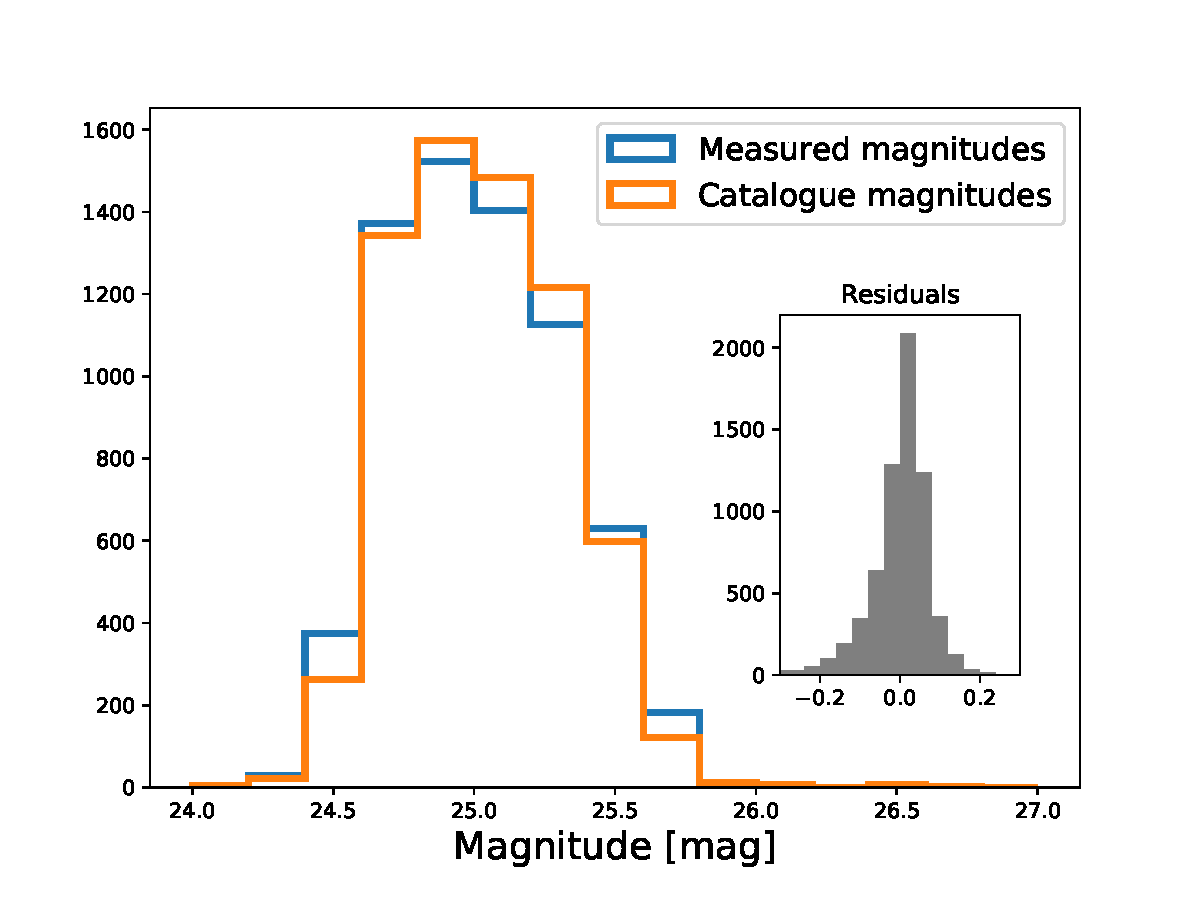
\includegraphics[trim={0.5cm 0 2cm 1.8cm},clip,width=0.45\textwidth]{Code/Saved_Figures/Mag_hist.pdf}
    \caption{The distribution of magnitudes pertaining to objects in the COSMOS field. In blue, the magnitude measurements found by running SEP is plotted. In orange the 2'' magnitudes reported in the COSMOS2020 Classic catalogue are displayed. In grey a residual plot is shown, mapping the difference between the measured and reported magnitude for each object.}
    \label{mag_hist}  
\end{wrapfigure}

The centroids of the sources found by SEP in the IRAC $ch1$ band can then passed to the software IRACCLEAN \cite{Hsieh_2012_IRACCLEAN} to model the IRAC $ch1$ emission. The centroids from the SEP algorithm and the total flux found from fixed aperture photometry is used to create point source models of the detected objects. The point source model is an approximation, since the light profiles of the galaxies will differ from a perfect point source. However, due to the low resolution of the IRAC images and their large point spread functions (PSF), much larger than the expected sizes of our candidates and of most distant objects, it is reasonable to use the point-like approximation. The COSMOS team used IRACCLEAN software and a similar approach as described above, but performed on both $ch1$ and $ch2$ in IRAC, to produce what we will refer to in this project as the classic residual map. There are, however, some limitations to aperture photometry and the residual map it produces, which is why we will also explore another approach of creating a residual map.

\subsubsection{Model-Based Photometry}
An alternative to aperture photometry is model-based photometry, a method from which the Farmer tool is developed. The Farmer tool \cite{Weaver_2020}, like the previous method, also starts out with a source detection algorithm (SEP) reporting the centroids of each source detected. Next it identifies particularly crowded regions where there are multiple objects nearby each other that could present overlapping flux. Contrary to the previous methods, these sources are modelled simultaneously. Furthermore this method does not require enforcing a fixed aperture size. Instead the total flux is determined by fitting an intrinsic light profile to the source, and integrating the area covered by the model below the surface. The Farmer tool fits a source to one of 5 models. Common for all of them is that they are parametrised using the centroid position of the source as a fixed parameter and the total flux as a free parameter. The models are:
\begin{enumerate}
    \item \textbf{Point Source} models are taken directly from the point spread function (PSF) used. It is similar to the method applied when using aperture photometry.
    \item \textbf{Simple Galaxy} models are circular symmetric, exponential light profile with a fixed 0.45’’ effective radius.
    \item \textbf{Exponential Galaxy} models are exponential light profiles. In addition to the common parameters these are parametrised also by effective radius, axis ratio and position angle.
    \item \textbf{DeVaucouleurs Galaxy} models are de Vaucouleurs light profiles. These models require similar parameters as the exponential galaxy model.
    \item \textbf{Composite Galaxy} models are combines a Exponential Galaxy profile with a DeVaucouleur Galaxy profile. The profiles are concentric, and the model, like the others, is therefore only parametrised by one pair of centroids coordinates. Each component is parametrised by the free parameters described in the two previous models. In addition there is a “fraction of total flux” parameter that distributes the flux between the two components.
\end{enumerate}

Except for the Point Source model, they can all be described analytically by changing the parameter $n$ in a 2d Sérsic profile. $n=1$ corresponds to a Exponential Galaxy and $n=4$ creates a De Vaucouleurs Galaxy. The general profile is given by \cite{1968adga_book} in eq. \ref{sersic},
\begin{equation}
   I(R) = I_e \cdot \exp \left(-b_n \cdot \left( \left( \frac{R}{R_e} \right)^{\frac{1}{n}} - 1\right) \right)
   \label{sersic}
\end{equation}
where $I_e$ is the intensity at the effective radius $R_e$ that encloses half of the total light from the model. The constant $b_n$ is defined from $n$, to make sure the total luminosity is obtained when integrating the profile. Since four models are all analytical, they can easily be integrated to obtain the total flux. The real challenge lies in choosing the right model and obtaining a converging fit. The Farmer tool includes a decision tree for selecting the most appropriate model type to fit a given source with. The models are tested in the order they are described above (1 to 5), and the quality of their residuals are ranked, so the best model is chosen. When the most appropriate model type is selected for all sources, optimisation of the free parameters is performed as the final step, so that the parameters chosen for one object will not directly affect the parameters of nearby objects. While this method does improve on some of the drawbacks from aperture photometry, it is next to impossible to make all model fittings converge. There are a few possible reasons for the failure to converge. Sometimes a bright source is simply not well described by a smooth profile. It could also be due to a very blended pair that was not successfully separated in the detection, and thus not described correctly by a single light profile. \\
With this process, the Farmer tool can provide us with the parameters needed for creating intrinsic light profiles of the sources detected in the image. The models describe how we expect the light to look intrinsically, but when the light is observed through a telescope it is warped due to the way the imaging system responds to a point source. A point spread function (PSF) describes the response of an imaging system to a point source, mapping how the light will appear in the image. Therefore, to create a residual image we need to model the objects as they would appear in the image. We obtain the final models from a convolution of the intrinsic light profiles with the PSF of the image. The residual map is then produced by subtracting the convolved models from the telescope image, carefully placing the models right according to the detected centroid coordinates. \\ \\
For the next part of the project we need a catalogue containing the coordinates and total flux of objects detected in the residual image. For this purpose we use SEP source detection and aperture photometry to estimate the total flux. This catalogue will likely contain different objects of various level of interest: spurious objects, left-over flux from subtracted sources due to imperfections in the residual image, and dropout galaxies.

\subsection{Classification with Semi-supervised Machine Learning}
In this thesis, we develop a semi-automated method of selecting NIR-dropout galaxies based on t-SNE \cite{Maaten_2008_tSNE} and kNN voting. This method uses as input: 4 telescope image cutouts of each galaxy in the sample, from respectively the $H$, $Ks$, $ch1$ and $ch2$ bands. The method is semi-supervised, and hence will need some parameter tuning along the way and some labels (to be defined in section 2.2.2). With this, the technique will predict whether each galaxy in the sample is a NIR dropout or not.

\subsubsection{Dimensionality Reduction with t-SNE}
As mentioned, the input that the method is given for each object in the sample is four small telescope images centred at the object in question. We use cutouts of the size $21\!\times\!21$ pixels, meaning that we in total will have $21\times21\times4=1764$ features for each object in the sample. Inherently, this is a very high-dimensional classification problem, and it is particularly difficult to produce meaningful predictions from, when the learning is unsupervised. A way to simplify the problem is embedding the high-dimensional data in a 2-d representation. There are many approaches to obtaining such an embedding, but for our purposes we will adopt the method of t-SNE, which has gained a lot of popularity since its release in 2008. A recent NBI paper \cite{Steinhardt_2020} proposed this novel technique for classification of galaxies from photometric data, which has inspired the approach applied here. In particular they used t-SNE to classify quiescent galaxies from their spectral energy distributions (SEDs). \\

t-SNE takes a set of high dimensional vectors, in this case the pixels originating from four different images, and computes the euclidean distance between each vector. From this it calculates a probability that two vectors should be considered neighbours. This probability considers the user-specified hyper parameter \textit{perplexity}, which determines the sizes of the neighbourhoods based on the density of the data in the respective regions. The hyper parameter can effectively be understood as a estimate for the number of neighbours that should be considered similar. Values between 1 and 50 are suggested by the author to be the most appropriate \cite{Maaten_2008_tSNE}. A low perplexity emphasizes local structure in the embedding, while a high perplexity will preserve more of the global structure of the samples. A universally good perplexity value cannot be determined, but should be selected manually for each data set. This is because the density of the objects varies depending on the sample size, and thus the number of optimal neighbours will vary. The perplexity is chosen, in this thesis, by performing the t-SNE embedding for various perplexities and determining which structure is best suited for the purpose of classifying dropouts. \\
t-SNE is stochastic in its nature, and will thus compute different embeddings for the same data set unless the same random seed is specified every time. To be able to reproduce our results, this was therefore implemented. Its stochastic nature lies in the fact that it will try out different configurations for the embedding and evaluate the probabilities, which it will try to improve in the next iteration. Due to the huge dimension of the data, this makes the process much faster, but also means that the embedding is not reversible, and new objects cannot be added individually to the embedding space. All data thus has to be given to the algortihm at once. We can specify the maximum number of iterations for the procedure, and the algorithm will output the number of iterations it actually used to produce the embedding. This means we can also use the number of iterations as a tool for choosing the right perplexity. If the number of iterations is smaller than the maximum number of iterations, this means the embedding has converged in the sense that it could not find a better configuration for the embedding during the next 300 iterations (since the default value for the parameter \textit{n\_iter\_without\_progress} is 300). \\
Since the t-SNE algortithm is a form of unsupervised machine learning, the embedding map will be produced without any direct knowledge of what a dropout galaxy looks like. It will however place objects it considers similar close to each other, even though the algorithm is unaware that the features are pixels from a series of telescope images. This is also one of the reasons t-SNE is so popular: the flexibility in its applications makes it a very powerful tool.

\subsubsection{Visual Classification of Tracers}
\begin{wrapfigure}{r}{0.4\textwidth}
    \centering %left, lower, right, upper
    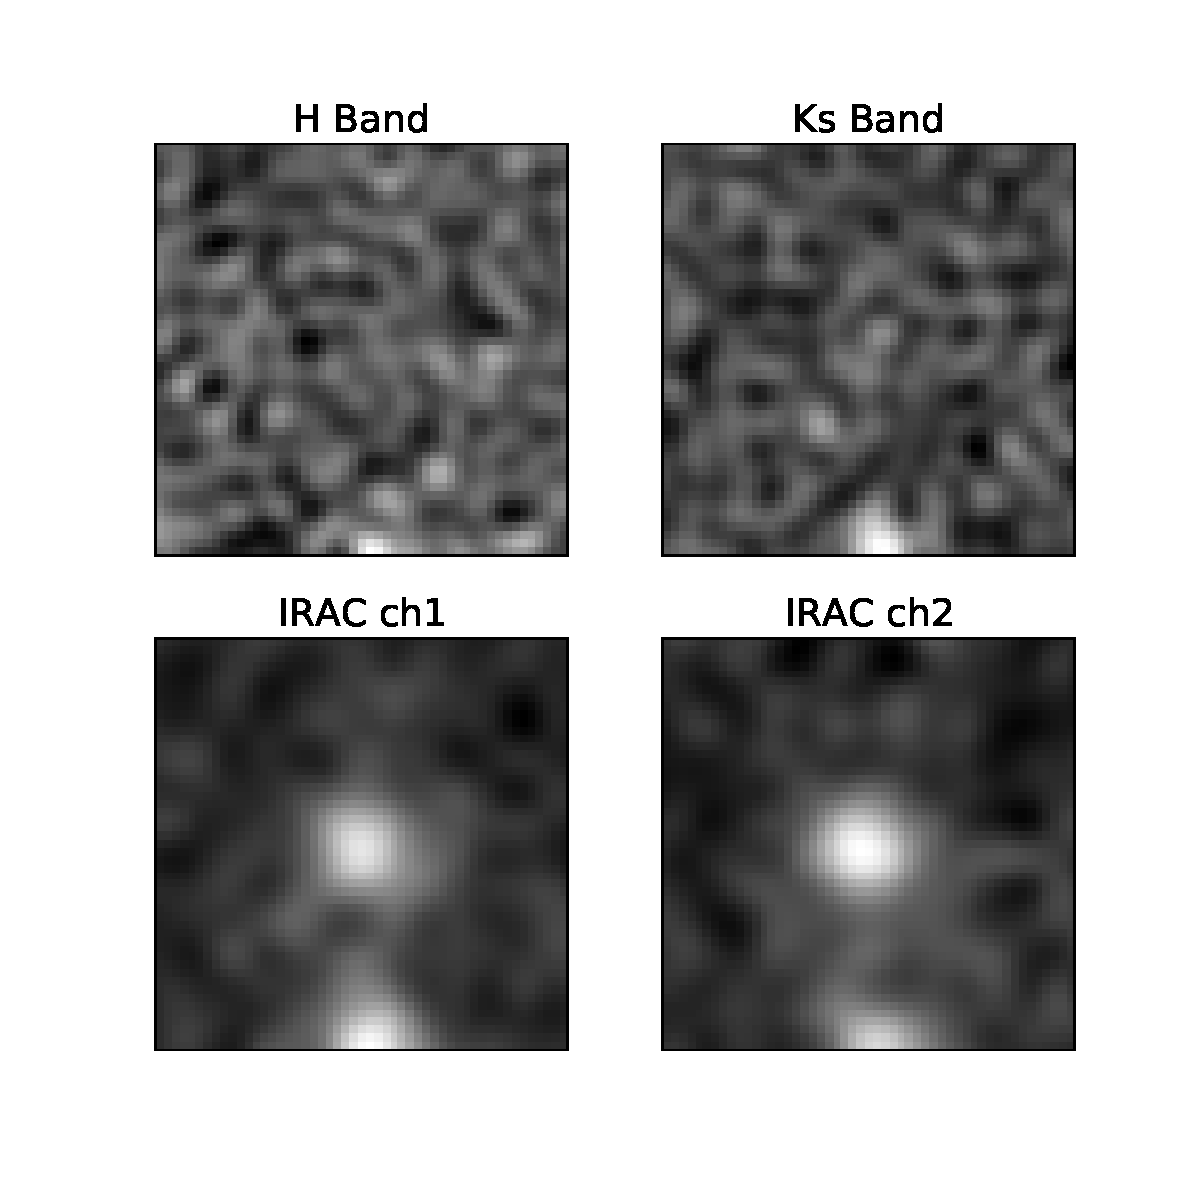
\includegraphics[trim={1cm 2.5cm 2cm 1.5cm},clip,width=0.38\textwidth]{Code/Saved_Figures/good_example.pdf}
    \caption{An example of a tracer for NIR-dropouts. The object is clearly visible in the IRAC bands, while it drops out in the NIR bands.}
    \label{tracer_example}  
\end{wrapfigure}
Thus far the machine learning has been completely unsupervised, but now that a 2-d representation of the sample is obtained, we need to understand in which region dropout galaxies are located with another method, since t-SNE, by itself, is not enough to produce predictions. As mentioned in section 2.2.1, t-SNE has no direct knowledge of the features it is mapping, and while it is able to place similar objects close to one another, it is not able to define which categories different regions belong to. Even if the the method performs extremely well for our purpose, in the sense that it would output 3+ tight clusters that are well separated from each other, it would still not be enough, since it would not know which cluster contains what. We say 3+ clusters here, since we know there will be at least three kinds of objects: spurious sources, leftover sources and dropout galaxies. \\
This is therefore where the semi-supervised learning has to enter our method. We select "tracers" in our sample, which are what is determined to be a reliable NIR-dropouts based on a visual inspection of the objects in the four bands. We look for objects that are visible in IRAC $ch1$ and $ch2$, and which do not appear in the NIR bands $H$ and $Ks$. Since the objects we look for are similar to those found in \cite{Alcalde_Pampliega_2019} and \cite{Wang_2019}, we can also use these as a reference. An example of which objects we would classify as a tracer is displayed in fig. \ref{tracer_example}. We can then map where the tracers are placed in the embedding by the t-SNE algorithm. If the tracers cluster well, this is a good indication of a promising region for finding NIR-dropouts. \\
For the method adopted in this thesis, we also need "anti-tracers", which are indicators of non NIR-dropouts. These are also selected from a visual inspection of the four bands, this time, however, we look for objects that look nothing alike the tracer displayed in fig. \ref{tracer_example}. \\ 
Since we devise the semi-supervised method for selecting NIR-dropouts in this thesis, we will also need to validate it. This means we need a sample of tracers and anti-tracers for producing predictions, and additionally a similar sample for validating. In case of future use of the method this is, however, not necessary, thus reducing the number of objects that has to be visually classified.

\subsubsection{Classification with kNN voting}
Now that we have an embedding that is more easily visualised and interpreted, and we have tracers and anti-tracers indicating the interesting regions and the non-interesting regions, we can construct the semi-supervised algorithm used to produce predictions on the sample. An object can either be classified as a NIR-dropout or a non NIR-dropout galaxy. The method takes basis in the principle of k nearest neighbours and voting. The code performing the classification is divided into the following modules:
\begin{enumerate}
    \item First, the distances between an unknown object and all tracers are computed, from which the k nearest tracers are selected (a range of values $1<k<50$ will be tested).
    \item The votes of the k neighbours are then collected. A neighbour that has been previously identified as a tracer will vote for a NIR dropout prediction, while an anti-tracer will vote against.
    \item It is checked if the fraction of positive votes is above the threshold $f_{min}$, which defines the minimum fraction required for predicting a dropout. In the implementation we will experiment different values of $f_{min}$, ranging from 0 to 1. 
    \item On behalf of the above, the predictions are computed.
\end{enumerate}
An alternate strategy would be collecting votes from all the neighbours within a fixed radius in the 2-d space. The choice of using nearest neighbours instead of this other option is based on two considerations. First of all the two dimensions of the t-SNE embedding are arbitrary, thus defining a physically meaningful radius is challenging. Furthermore, the embedding represents an approximation of the higher dimensional distribution of objects, and therefore we cannot be certain that a euclidean distance in one region of the embedding is consistent with the distance measured in another region. Assuming a uniform density of objects in the embedding, using the k nearest neighbours, would in turn provide a more consistent voting. By introducing the threshold $f_{min}$, we are able to modify our selection of NIR dropouts based on the desired balance of quality and quantity. One can then select a parameter of $f_{min}$ that identifies fewer, more robust dropout candidates or be less conservative and obtain predictions of more NIR-dropouts that in turn may be less reliable. \\ \\
We will evaluate the performance of the model based on the purity of the sample, defined as $TP/(TP+FP)$ where TP is the number of true positives and FP is the number of false positives. We will also produce a receiver operator characteristic (ROC) curve, useful for visualising the performance for different values of $f_{min}$, and typically an adopted score measure in machine learning. The ROC curve is defined as the true positive rate (TPR) as a function of the false positive rate (FPR) \cite{FAWCETT2006861_ROC}.